\documentclass{jsarticle}

\usepackage[dvipdfmx]{graphicx}
\usepackage{multicol}
\usepackage{here}
\usepackage{geometry}
\geometry{left=25mm,right=25mm,top=20mm,bottom=20mm}
\usepackage{url}

\title{情報通信プロジェクト G班中間報告書}
\author{13EC602 郭柏辰, 14EC004 飯田頌平, 14EC552 陳玉皓, 14EC602 劉宇航}

\begin{document}

  \maketitle
  
  %\begin{multicols}{2}
  
    \section{企画の目的}
    
      % 背景
      既存の天気予報は都市毎にしか見ないものであったり、
      雨雲の動きを生データで実況するものが多く、
      気象予報士でもない一般人が特定の位置の天気を予報するには向いていない。
      
      % 目的
      そのため、センサを活用して局地的な天気を予測できる
      IoTデバイスに需要があると考えられる。
    
    \section{構成}
    
      % 問題設定
      局地的な情報を計測する必要があるため、
      センサは持ち運びができるものでなくてはならない。
      
      センサが測定したデータを取り出す部品も、同様にコンパクトである必要がある。
      
      % 使用機材
      そこで、データ取得を行う部品にRaspberryPiを採用する。
      RaspberryPiは名刺ほどの小型のコンピュータであり、
      MicroSDカードにシステムやデータを保存する。
      
      RaspberryPiはGPIO端子を通してI2C(Inter Integrated Circuit)接続を行えるため、
      I2Cに対応したセンサであるBME-280を用いて、温度・湿度・気圧を計測する。
      
      こうして小型の部品を活用することで、どこにでも天気予報機を持ち運んで
      天候のデータを測定することができる。
      
      測ったデータから天気予報を行うには、ニューラルネットワーク\cite{Schmidhuber}という
      アルゴリズムを採用する。
      
      RaspberryPiはLinuxベースのOSで動いているため、
      Pythonプログラムで実装したニューラルネットワークを使って予測を行える。
      
      予測結果は、RaspberryPiのGPIO端子に接続するタイプの
      小型ディスプレイを通してユーザに伝えられるようにする。
    
      以上のことから、構成部品をまとめたものを下に示す。
    
      \begin{center}
        \begin{table}[H]
          \centering
          \caption{構成部品一覧}
          \begin{tabular}{|c|c|r|} \hline
            種別 & 名称 & 値段\   \\ \hline \hline
            マイコン & RaspberryPi3 ModelB & 5.600円(a) \\
            MicroSDカード & SanDisk Ultra 40MB/s 8GB & 798円(b) \\
            温湿度・気圧センサ & BME-280 モジュール & 1,080円(a) \\
            ディスプレイ & AE-AQM0802 モジュール & 700円(a) \\
            オス-オスジャンパ & 10cm20本セット & 180円(a) \\
            オス-メスジャンパ & 15cm(赤)10本セット & 220円(a) \\
            ブレッドボード & BB801 & 200円(a) \\ \hline \hline
             &                 合計 & 8,778円 \\ \hline
          \end{tabular}
        \end{table}
        {\scriptsize 価格は(a)秋月電子(b)amazon調べ}
      \end{center}
    
    \section{内部仕様}
    
      \subsection{ブロック構成図・回路図}
      
        ブロック構成図を\ref{fig:block}に、
        回路図を図\ref{fig:circuit}に示す。
      
        \begin{figure}[htbp]
          \begin{center}
            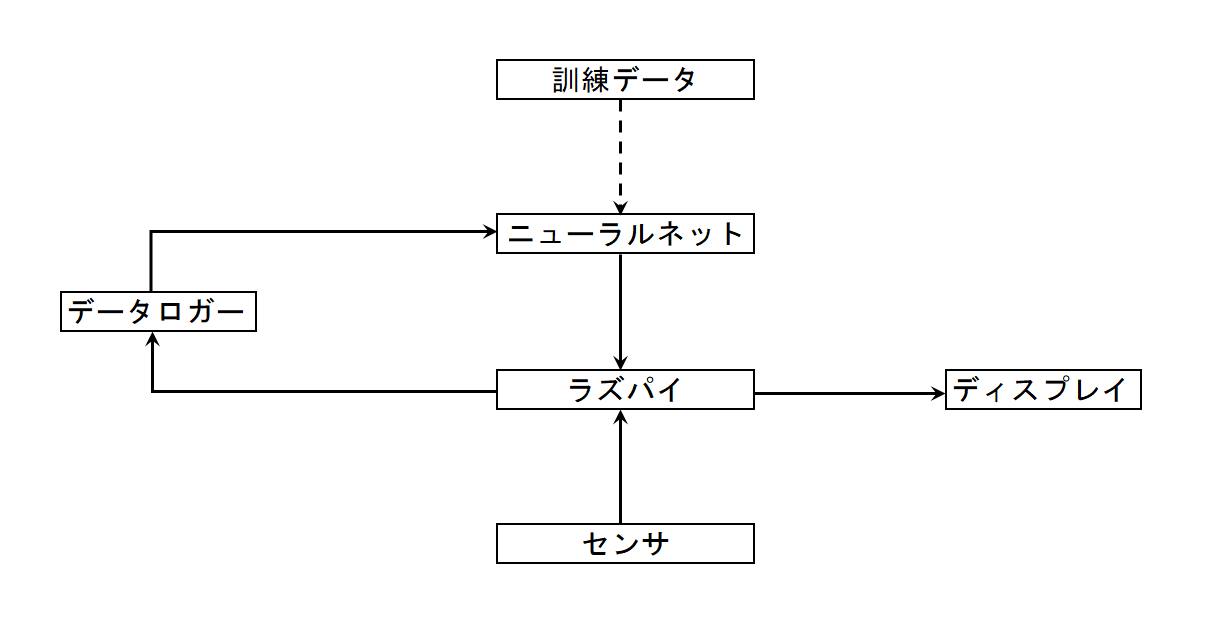
\includegraphics[clip,width=10.0cm]{img/block}
            \caption{ブロック構成図}
            \label{fig:block}
          \end{center}
        \end{figure}

        \begin{figure}[htbp]
          \begin{center}
            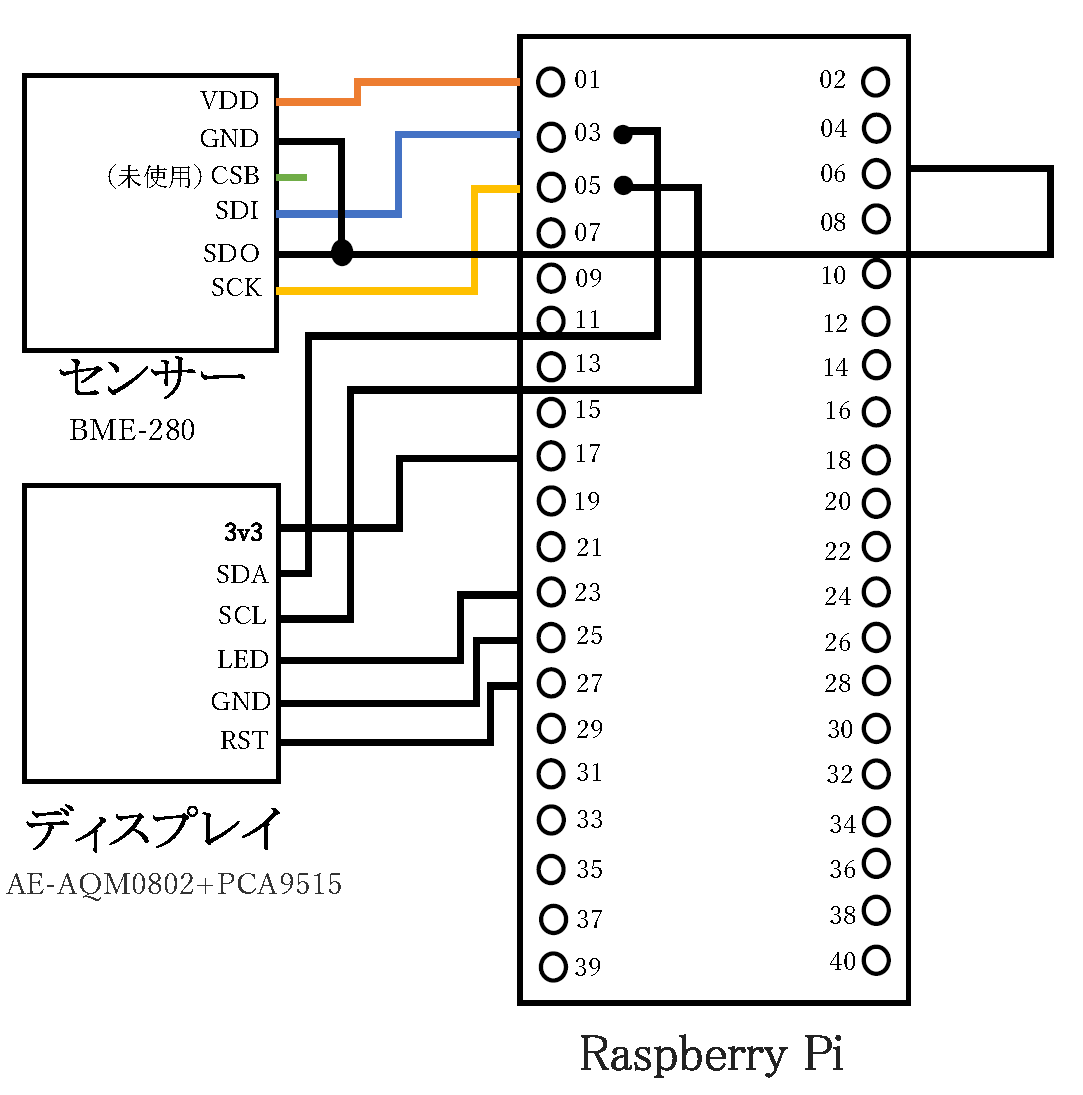
\includegraphics[clip,width=7.0cm]{img/circuit}
            \caption{回路図}
            \label{fig:circuit}
          \end{center}
        \end{figure}
        
        RaspberryPiにはI2Cでセンサとディスプレイが接続されている。
        センサおよびディスプレイはブレッドボード上に配置される。
        
    
      \subsection{ソフトウェア}
      
        \subsubsection{OS}
        
          RaspberryPiを動かすOSには、Raspbianを採用する。
          これはRaspberryPiが公式にサポートしているOSであり、
          Ubuntuベースで作られているため、
          bashを用いて通常のLinuxのようにソフトウェアを動かせるためだ。
          
        \subsubsection{センサ読み取り}
        
          センサが取得したデータを読み取るソフトには、
          センサ・モジュールの販売元である
          SwitchScienceが提供しているプログラムを用いる。
          読み取りプログラムはPythonでラップされており、
          Python上のstr(文字列)形式でデータを取得することができる。
          さらにこのコードを改変して、読み取ったデータを
          天気予報用のプログラムに送信するようにする。
          
          また、
          定期的なデータの取得にはbashコマンドのcrontabというものを用いる。
          これによって、
          一時間毎にデータを読み取るコマンドを自動的に実行できる。
          
        \subsubsection{天気予報}
        
          天気予報を行うプログラムとして、
          Pythonでニューラルネットワークを実装したコードを用いる。
          
          Pythonは深層学習用のライブラリを多数有しており、
          ニューラルネットワークを用いた
          プログラムの実装に向いているためだ。
          
          実装にあたって、深層学習用ライブラリのKerasを採用する。
          Kerasはバックエンドのライブラリに数値計算の処理を任せており、
          勾配法の実装などの詳細な点を無視しながら
          比較的簡単にニューラルネットワークを実装できる。
          
          今回用いるものはLSTM\cite{Hochreiter}と呼ばれるモデルだが、
          これは時系列の情報を学習することができ、
          通常のニューラルネットワークよりも
          時間の変化による予測値の変化に敏感になるためだ。
          
          一般的に、ニューラルネットワークによる予測には、
          事前に学習用データを用いてネットワークの訓練を行う必要がある。
          学習用データには、気象庁が用意しているCSVデータを採用する。
          これは不要な情報が多々含まれているため、
          Pythonプログラムによって必要な情報だけを抽出する。
          
          抽出する情報は、
          一日あたりの平均温度・平均湿度・平均気圧・降水量の4項目で、
          これらを一年分用意する。
          降水量についてはしきい値を取り、一定量の降水量があったときに
          雨天であると判定し、ブール値でフラグを立てるように変換する。

          そうして生成されたデータを逐次的にLSTMに入力し、
          誤差逆伝播法\cite{Le}のアルゴリズムによって
          天気予報に適したモデルを生成する。
          天気予報モデルは、
          センサから得た温度・湿度・気圧の3次元のデータに基いて、
          未来の降水確率を出力する。

          なお、現段階ではRaspberryPiに組み込んで使用するため、
          マシンパワーに不安がある。
          そのため、簡単なネットワークを組むことにした。
          具体的には、以下の構成からなるニューラルネットである。

          \begin{itemize}
            \item LSTM層,隠れユニット数:10
            \item 全結合層,ユニット数:10
            \item 活性化関数,シグモイド
            \item 誤差関数,二乗誤差
          \end{itemize}

          最適化手法は勾配降下法の一種である
          RMSProp\cite{Hinton}を採用した。

          また、活性化関数については、LSTM内の各ユニット間に
          シグモイド関数とハイパボリック・タンジェント関数を用い、
          全結合層と出力層の間にはシグモイド関数を用いている。
          出力層の前の非線形関数がシグモイドなのは、
          出力値を確率値として表現するためである。

          
          %天気予報用モデルはふたつのネットワークからなる。
          %第一のネットワークは、回帰によって未来のデータを予測する。
          %具体的には、温度・湿度・気圧の3次元のデータについて、
          %観測時点のデータとその12時間前までのデータを入力することで、
          %次の12時間分の各データを予測する。
          %第二のネットワークは、予測されたデータを用いて、
          %未来の各時点での降水確率を出力する。
          
        \subsubsection{ディスプレイ}
        
          採用したディスプレイAE-AQM0802は、RaspberryPiからbashコマンドで動作させることができる。
          Pythonのsubprocessモジュールからbashを操作することで、
          間接的にPythonプログラム上からディスプレイの操作ができる。
      
    \newpage
    \section{外部仕様}
    
      \subsection{外観}
        \begin{figure}[htbp]
          \begin{center}
            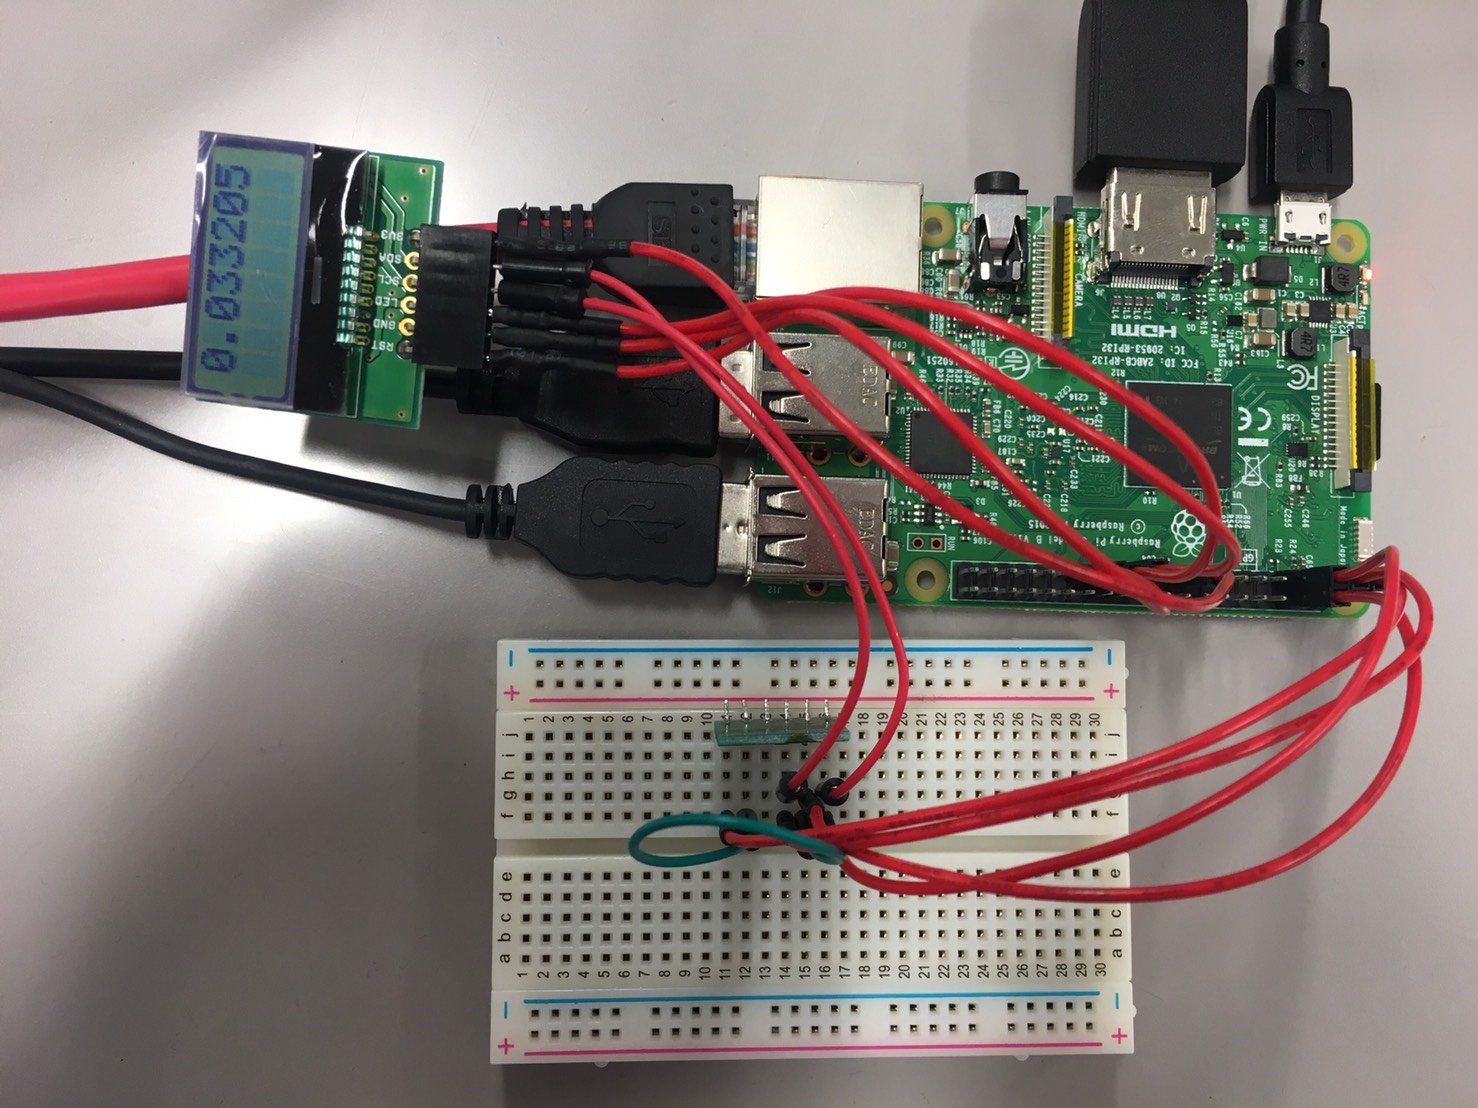
\includegraphics[clip,width=7.0cm]{img/finish}
            \caption{現在の外観}
            \label{fig:finish}
          \end{center}
        \end{figure}

        \begin{figure}[htbp]
          \begin{center}
            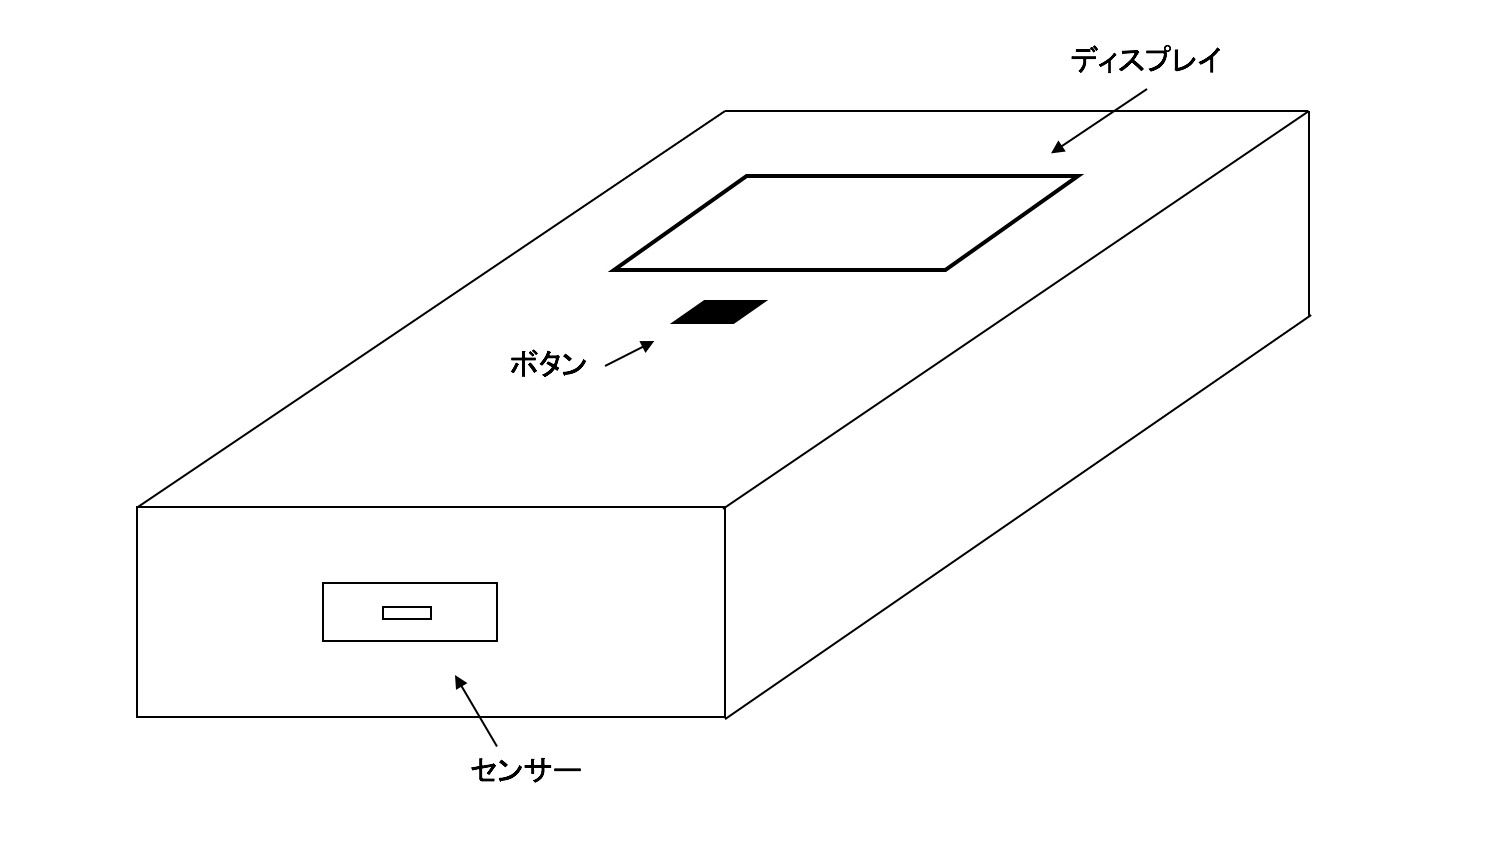
\includegraphics[clip,width=7.0cm]{img/finish2}
            \caption{完成予想図}
            \label{fig:finish2}
          \end{center}
        \end{figure}

        本デバイスの外観を図\ref{fig:finish}に示す。
        予算に余裕があるならば、
        さらに図\ref{fig:finish2}のようにケースで覆い、
        ボタンを押すことで予測を開始できるようにする。

      \subsection{使用方法}
        本デバイスの使用方法は、以下の手順に則る。
        
        \begin{enumerate}
          \item デバイスの電源を入れて、起動する
          \item デバイスを適当な観測箇所に設置する
          \item ディスプレイに出力された天気予報を確認する
        \end{enumerate}
        
        センサによる測定を行う上で、屋外での動作が見込まれているが、
        予算の都合上、
        雨よけのケースや携帯型のバッテリーを不採用にしたので、
        実際の運用では窓の近くに設置する形が想定される。
        
        ディスプレイの出力値は、単純に確率を数値で表したものと、
        その確率をどう判断すべきかの目安となる文字列を表すことにする。
        これによって、ユーザは傘を持っていくかどうかという、
        もっとも重要な情報を即座に判断できるようになる。

        また、実際に運用する際には、
        観測地点の温湿度データを記録し続ける必要がある。
        そのため、据え置き型のデバイスとして使うことになる。
        初使用時など、十分なデータを記録出来ていない場合には、
        気象庁が公開している過去の観測データを
        代わりに使用した予測を行うようにする。

    \section{作業計画}
      \subsection{現在の進捗状況}
        当報告書の内部仕様・外部仕様に記載した点は、
        一通り完了した。
        具体的には、

        \begin{itemize}
          \item RaspberryPiのセットアップ
          \item センサーによるデータの取得
          \item ディスプレイへの表示
          \item ニューラルネットによる予測
        \end{itemize}

        ここまでが一通り完了し、
        ターミナルからコマンドを打つと、
        センサから取得した値を用いた予測結果が
        ディスプレイに表示されるようになっている。

        なお、現在の予測精度はおよそ70\%である。
        気象庁の発表によると、2015年の
        降水の有無の的中率は85\%を越える\cite{jma}ので、
        当デバイスの目標精度も85\%とする。

      \subsection{今後のスケジュール}

        \begin{center}
          \begin{table}[H]
            \centering
            \caption{スケジュール表}
            \begin{tabular}{|c|l|} \hline
              \hspace{5mm}日付\hspace{5mm} & \hspace{30mm}予定 \\ \hline \hline
              7/31 & 報告書提出 \\
              8/15 & モジュールテスト:温湿度ログ管理 \\
              8/29 & モジュールテスト:クライアント・サーバ間通信 \\
              9/12 & モジュールテスト:
                        ディープ・ニューラルネットによる予測 \\
              9/19 & 実装テスト、追加目標の定義 \\
              9/26 & タスク消化 \\
              10/3 & 以後、予備日 \\ \hline
            \end{tabular}
            \label{tb:schedule}
          \end{table}
        \end{center}

        表\ref{tb:schedule}に今後の作業計画を示す。
        9/19までは実機に触れないので、
        それまでは二週間の間隔で各モジュールのテストを行う。
        各モジュールテストの詳細を以下に示す。
        \begin{description}
          \item[温湿度ログ管理]
            cronを使ったログの自動取得、保存、読み出しを、
            センサの値の代わりにダミーデータを用いて確認する。
          \item[クライアント・サーバ間通信]
            研究室にあるLinuxサーバとノートパソコンの間で、
            pythonコード上のソケット通信によるデータのやり取りを確認する。
          \item[ディープ・ニューラルネットによる予測]
            現在はLSTMを一層用いて、一日の平均の温湿度から
            翌日の降水確率を予測している。
            これに対し、複数のLSTMと時間単位の温湿度から、
            数時間後の降水確率を予測できるようにする。
        \end{description}
      
      \newpage
      \subsection{班内での分担}
        以下のように班内で作業を分担する。
        \begin{description}
          \item[飯田]ニューラルネット関連プログラム
          \item[陳]センサ・ディスプレイ関連プログラム
          \item[劉・郭]実機での配線、部品調達、図面作成など
        \end{description}

    \section{総括}
      中間報告時点で、計画通りに作業が進んでいる。
      精度や構成などはより改善する余地が残っており、
      今後はそれらに力を入れる予定だが、
      既に単独のIoTデバイスとして使用できるだけの完成度に達している。
      
  
  \begin{thebibliography}{9}
    \bibitem{Schmidhuber} Schmidhuber, Jürgen. "Deep learning in neural networks: An overview." Neural networks 61 (2015): 85-117.
    \bibitem{Hochreiter} Hochreiter, Sepp, and Jürgen Schmidhuber. "Long short-term memory." Neural computation 9.8 (1997): 1735-1780.
    \bibitem{Le} LeCun, Y., Boser, B., Denker, J.S., Henderson, D., Howard, R.E., Hubbard, W., \& Jackel, L.D. (1990). Handwritten digit recognition with a back-propagation network.Advances in Neural Information Processing Systems, 2, 396–404, Morgan Kaufman.
    \bibitem{Hinton} Geoffrey Hinton, Nitish Srivastava, Kevin Swersky. "Neural Network for Machine Learning - Lecture 6a Overview of mini-batch gradient descent"
    \bibitem{jma} 気象庁. "天気予報の精度検証結果" \url{http://www.data.jma.go.jp/fcd/yoho/kensho/yohohyoka_top.html}
  \end{thebibliography}
    
  %\end{multicols}

\end{document}
